\documentclass[]{AVSSimReportMemo}
\usepackage{AVS}
\usepackage{colortbl}
\usepackage{float}


\newcommand{\ModuleName}{locationPointing}
\newcommand{\subject}{Guidance Module for Ground Location Pointing}
\newcommand{\status}{Initial Version}
\newcommand{\preparer}{L. Redner}
\newcommand{\summary}{Generate the attitude reference to perform a constant pointing towards a static ground location}


\begin{document}

\makeCover


%
%	enter the revision documentation here
%	to add more lines, copy the table entry and the \hline, and paste after the current entry.
%
\pagestyle{empty}
{\renewcommand{\arraystretch}{2}
\noindent
\begin{longtable}{|p{0.5in}|p{4.5in}|p{1.14in}|}
\hline
{\bfseries Rev}: & {\bfseries Change Description} & {\bfseries By} \\
\hline
Draft & initial copy & L. Redner \\
\hline

\end{longtable}
}

\newpage
\setcounter{page}{1}
\pagestyle{fancy}

\tableofcontents
~\\ \hrule ~\\

\section{Module Input and Output}
Table \ref{tab:inputNavTable} shows the Spacecraft State input message.
\begin{table}[h!]
	\centering
	\caption{Input Spacecraft States Message}
	\begin{tabular}{|l|l|l|p{3in}|}
		\hline
		\rowcolor{BrickRed}
		\textcolor{white}{Name} & \textcolor{white}{Type} & 
		\textcolor{white}{Length} & 
		\textcolor{white}{Description}  \\ \hline
		$\bm{r}_{B/N}$ & double [] & 3 & 
		Position vector of the spacecraft body-point with respect to the inertial frame in inertial frame components 
		($\leftexp{N}{\bm{r}}_{B/N}$) . \\ \hline
		$\bm{\omega}_{B/N}$ & double [] & 3 & 
		Angular velocity vector of the spacecraft point with respect to the inertial frame in body frame components 
		($\leftexp{B}{\bm{\omega}}_{B/N}$). \\ \hline
	\end{tabular}
	\label{tab:inputNavTable}
\end{table}

Table \ref{tab:inputCelTable} shows the Ground State input message.
\begin{table}[h!]
	\centering
	\caption{Input Ground State Message}
	\begin{tabular}{|l|l|l|p{3in}|}
		\hline
		\rowcolor{BrickRed}
		\textcolor{white}{Name} & \textcolor{white}{Type} & 
		\textcolor{white}{Length} & 
		\textcolor{white}{Description}  \\ \hline
		$\bm{r}_{L/N}$  & double [] & 3 & 
		Position vector of the ground location with respect to the inertial origin in the inertial frame ($\leftexp{N}{\bm{r}}_{L/N}$). \\ \hline
	\end{tabular}
	\label{tab:inputCelTable}
\end{table}

Table \ref{tab:inputCelTable} shows the user specified inputs required.
\begin{table}[h!]
	\centering
	\caption{User Specified Input}
	\begin{tabular}{|l|l|l|p{3in}|}
		\hline
		\rowcolor{BrickRed}
		\textcolor{white}{Name} & \textcolor{white}{Type} & 
		\textcolor{white}{Length} & 
		\textcolor{white}{Description}  \\ \hline
		$\hat{\bm{p}}$  & double [] & 3 & 
		Satellite vector that will be aligned to point at the ground location. \\ \hline
	\end{tabular}
	\label{tab:inputCelTable}
\end{table}


Table \ref{tab:outputTable} shows the Attitude Guidance output message of the module locationPointing.
\begin{table}[h!]
	\centering
	\caption{Output Attitude Guidance Message}
	\begin{tabular}{|l|l|l|p{3in}|}
		\hline
		\rowcolor{BrickRed}
		\textcolor{white}{Name} & \textcolor{white}{Type} & 
		\textcolor{white}{Length} & 
		\textcolor{white}{Description}  \\ \hline
		$\sigma_{B/R}$ & double [] & 3 & Current attitude error estimate of B relative to R.
		 \\ \hline
		$\omega_{B/R}$ & double [] & 3 & 
		 Current body error estimate of B relative to R in B frame components ($\leftexp{B}{\omega_{B/R}}$).
		 \\ \hline
		${{\omega}_{R/N}}$ & double [] & 3 & Reference frame rate vector of R relative to N in B frame components
	    ($\leftexp{B} {{\omega}_{R/N}}$).	\\ \hline
		$ {\dot{\omega}_{R/N}}$ & double [] & 3 & Reference frame inertial body acceleration of R relative to N in B frame components
			($\leftexp{B} {\dot{\omega}_{R/N}}$).\\ \hline
	\end{tabular}
	\label{tab:outputTable}
\end{table}
\newpage




\section{Introduction}
In this module, the output attitude guidance message acts to point a prescribed satellite vector toward a static ground location. An example formulation of this problem is shown below.\\
% ADD FIGURE OF FORMULATION HERE
\begin{figure}[H]
    \centering
    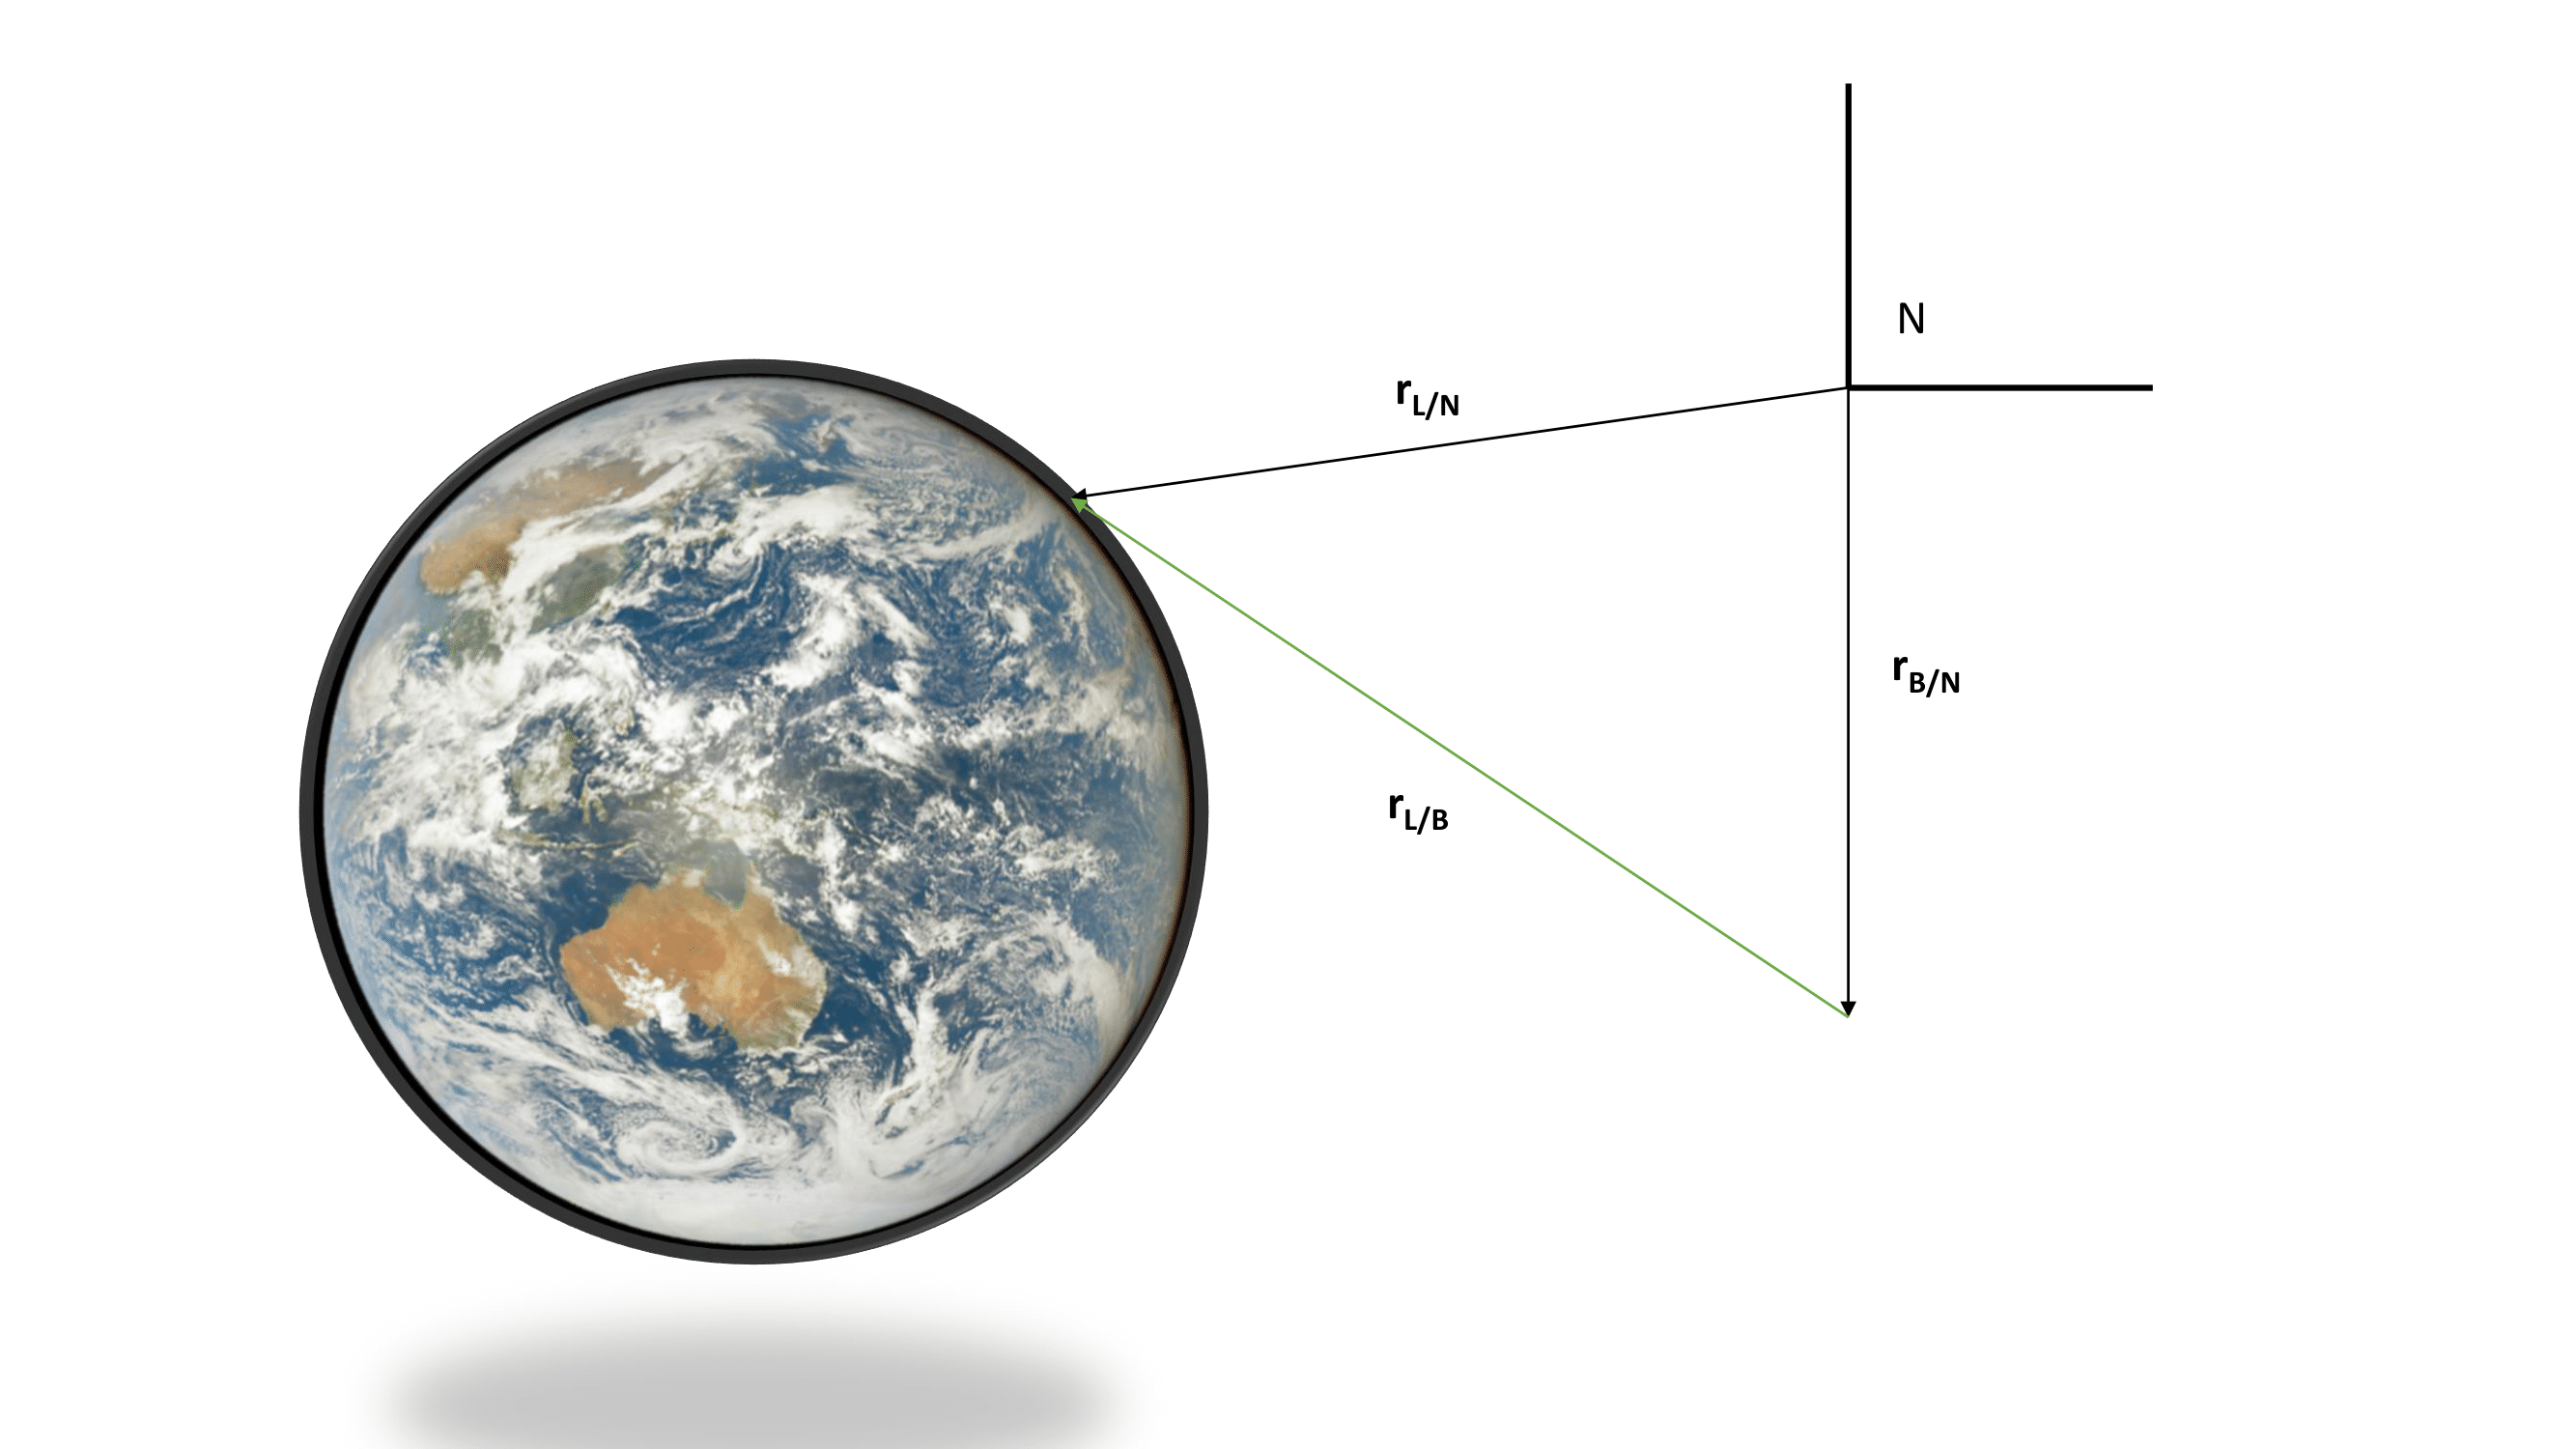
\includegraphics[width = 0.8\textwidth]{Figures/Problem_formulation.png}
    \caption{Problem formulation}
    \label{fig: formulation}
\end{figure}
The position of the spacecraft relative to the ground location is calculated by the following simple subtraction:
\begin{equation}
    \bm{\bar{r}_{L/B}} = \bm{\bar{r}_{L/N}} - \bm{\bar{r}_{B/N}}
\end{equation}
From this, the eigen axis is computed using the value calculated above and the user given satellite pointing vector.
\begin{equation}
	\label{eq:e}
	\bm{\hat{e}} = \frac{\bm{\hat{p}} \times \bm{\bar{r}_{L/B}}}{|\bm{\hat{p}} \times \bm{\bar{r}_{L/B}}|}
\end{equation}
Next, $\phi$ was calculated again using the pointing vector and the relative position of the ground location w.r.t the spacecraft:
\begin{equation}
	\label{eq:phi}
	\bm \phi = \arccos{\frac{\bm{\hat{p}} \cdot \bm{\bar{r}_{L/B}}}{|\bm{\bar{r}_{L/B}}|}}
\end{equation}
The current attitude error estimate of B relative to R (an output of the module) is computed using the above intermediate value:
\begin{equation}
	\label{eq: sigmaBR}
	\bm{\sigma_{R/B}} = \tan{\frac{\bm \phi}{4}}\bm{\hat{e}}
\end{equation}
$\sigma_{B/R}$ is the negative of $\sigma_{R/B}$, as shown below:
\begin{equation}
    \bm{{\sigma}_{B/R}} = - \bm{{\sigma}_{R/B}}
\end{equation}
A basic finite difference was used to calculate the time derivative of $\sigma$. Only two consecutive data points were used for the computation over the uniform time-step between them:
\begin{equation}
	\label{eq: dsigmaBR}
	\bm{\dot{\sigma}_{R/B}} = \frac{\Delta\bm{\sigma_{R/B}}}{\Delta t}
\end{equation}

At which point we can calculate the angular velocity required in the output message:
\begin{equation}
	\label{eq: omegaRB}
	\bm{\omega_{R/B}} = 4\bm{\dot{\sigma}_{R/B}}B(\bm{{\sigma}_{R/B}})^{-1}
\end{equation}
Where B inverse is computed using the following:
\begin{equation}B^{-1} = \frac{1}{|\bm{\sigma_{R/B}}|^2}
\begin{bmatrix}
    1 - |\bm{\sigma}| + 2 \bm{\sigma}_0^2     & 2  (\bm{\sigma}_0  \bm{\sigma}_1 + \bm{\sigma}_2) &2  (\bm{\sigma}_0  \bm{\sigma}_2 - \bm{\sigma}_1) \\ 2  (\bm{\sigma}_1  \bm{\sigma}_0 - \bm{\sigma}_2) & 1 - |\bm{\sigma}| + 2  \bm{\sigma}_1 \bm{\sigma}_1 & 2 (\bm{\sigma}_1  \bm{\sigma}_2 + \bm{\sigma}_0)\\2  (\bm{\sigma}_2 \bm{\sigma}_0 + \bm{\sigma}_1) & 2 (\bm{\sigma}_2 \bm{\sigma}_1 - \bm{\sigma}_0) & 1 - |\bm{\sigma}| + 2 \bm{\sigma}_2 \bm{\sigma}_2
\end{bmatrix}
\end{equation}
The angular velocity of the reference frame vector relative to the inertial frame in B frame components is then computed using the values calculated above.
\begin{equation}
	\label{eq: omegaRN}
	\bm{\omega_{R/N}} = \bm{\omega_{R/B}} + \bm{\omega_{B/N}}
\end{equation}
Finally, the angular acceleration of R relative to N is computed using a finite difference of the angular velocity values over 1 time-step.
\begin{equation}
	\label{eq: domegaRN}
	\bm{\dot{\omega}_{R/N}} = \frac{\Delta\bm{\omega_{R/N}}}{\Delta t}
\end{equation}


\bibliographystyle{unsrt}
\bibliography{references}

\end{document}
